\documentclass{standalone}

\usepackage{tikz}
\usetikzlibrary{cd}
\usetikzlibrary{calc}
\usepackage{pgfplots}

\usepackage{ifthen}

\usepackage{amsmath}

\begin{document}
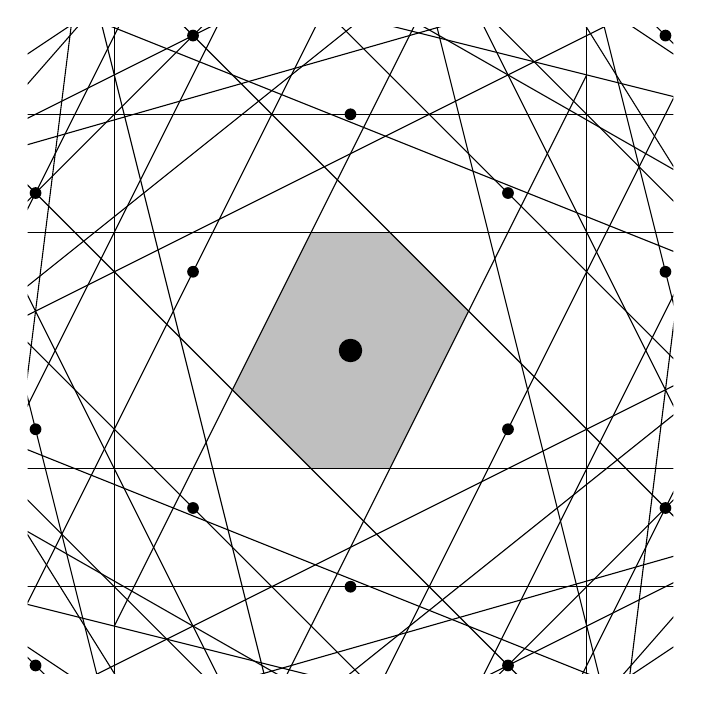
\begin{tikzpicture}
    \clip (-4.1,-4.1) rectangle + (8.2,8.2);
    \draw[draw=none,fill=lightgray] (-1.5, -0.5) -- (-0.5, -1.5) -- (0.5, -1.5) -- (1.5, 0.5) -- (0.5, 
    1.5) -- (-0.5, 1.5);
    \foreach \x in {-4,...,4}
    \foreach \y in {-4,...,4}{
    \ifthenelse{\x=0 \AND \y=0}{\node at ({\x *2},{\x*(-1) + \y *3})[circle,fill,inner sep=3pt]{};}
    {
    \draw[samples=3, domain=-4:4, smooth, variable=\t]
    plot ({(\x * 2) / 2 + (\x*(-1) + \y *3) / 2 * \t}, {(\x*(-1) + \y *3) / 2 - (\x *2) / 2 * \t});
    \node at ({\x *2},{\x*(-1) + \y *3})[circle,fill,inner sep=1.5pt]{};
    }
    }
\end{tikzpicture}
\end{document}